\section{User study}
Quantitative evaluation for texture synthesis is a particularly
challenging task as there is no single correct output when 
synthesizing new samples of a texture.
Like in other image generation tasks (\eg, rendering), 
human perception is ultimately the most important measure.
Thus, we performed a user study to evaluate the perceived 
realism of our synthesized textures.

Similar to previous image synthesis work (\eg, \cite{chen2017}), 
we conducted a perceptual experiment with human observers to 
quantitatively evaluate our synthesis results.
We employed a forced-choice evaluation on Amazon Mechanical
Turk (AMT) with 200 different users. Each user performed 59
pairwise comparisons between a synthesized dynamic texture and 
its target.
Users were asked to choose which appeared more realistic
after viewing the textures for an exposure time sampled
randomly from discrete intervals between 0.3 and 4.8 seconds.
Measures were taken to control the experimental conditions and
minimize the possibility of low quality data.
See the supplemental material for further experimental details
of our user study.

For comparison, we constructed a baseline by using the 
flow decode layer in the dynamics loss of Eq.\ \ref{eq:dynloss}.
This corresponds with attempting to mimic the optical flow 
statistics of the texture directly.
Textures were synthesized with this model and the user study
was repeated with an additional 200 users.
To differentiate between the models, we label ``Flow decode layer'' 
and ``Concat layer'' in the figures to describe our baseline and 
final model, respectively.

The results of this study are summarized in
Fig.\ \ref{fig:pairwise_alltextures} which shows user accuracy in
differentiating real versus generated textures as a function of
time for both methods.
Overall, users are able to correctly identify the real texture
$66.1\% \pm 2.5\%$ of the time for brief 
exposures of 0.3 seconds.
This rises to $79.6\% \pm 1.1\%$ with exposures of 1.2 seconds 
and higher.
Note that ``perfect'' synthesis results would have an accuracy
of $50\%$, indicating that users were unable to differentiate 
between the real and generated textures and higher accuracy 
indicating less convincing textures.

The results clearly show that the use of the concatenation 
layer activations is far more effective than the flow decode 
layer.
This is not surprising as optical flow alone is known to be 
unreliable on many textures, particularly those with
transparency or chaotic motion (\eg, water, smoke, flames, etc.).
Also evident in these results is the time-dependant nature of 
perception for textures from both models.
Users' ability to identify the generated texture improved as 
exposure times increased to 1.2 seconds and remained relatively 
flat for longer exposures.

To better understand the performance of our approach,
we grouped and analyzed the results in terms of
appearance and dynamics characteristics.
For appearance we used the taxonomy
presented in \cite{lin2006quantitative} and grouped textures as
either regular/near-regular (\eg, periodic tiling and brick wall), 
irregular (\eg, a field of flowers), or
stochastic/near-stochastic (\eg, tv static or water).
For dynamics we grouped textures as either 
spatially-consistent (\eg, closeup of rippling sea water) or 
spatially-inconsistent (\eg, rippling sea water juxtaposed 
with translating clouds in the sky).
Results based on these groupings can be seen in
Fig.\ \ref{fig:pairwise_grouped}.

\begin{figure}[t]
	\centering
    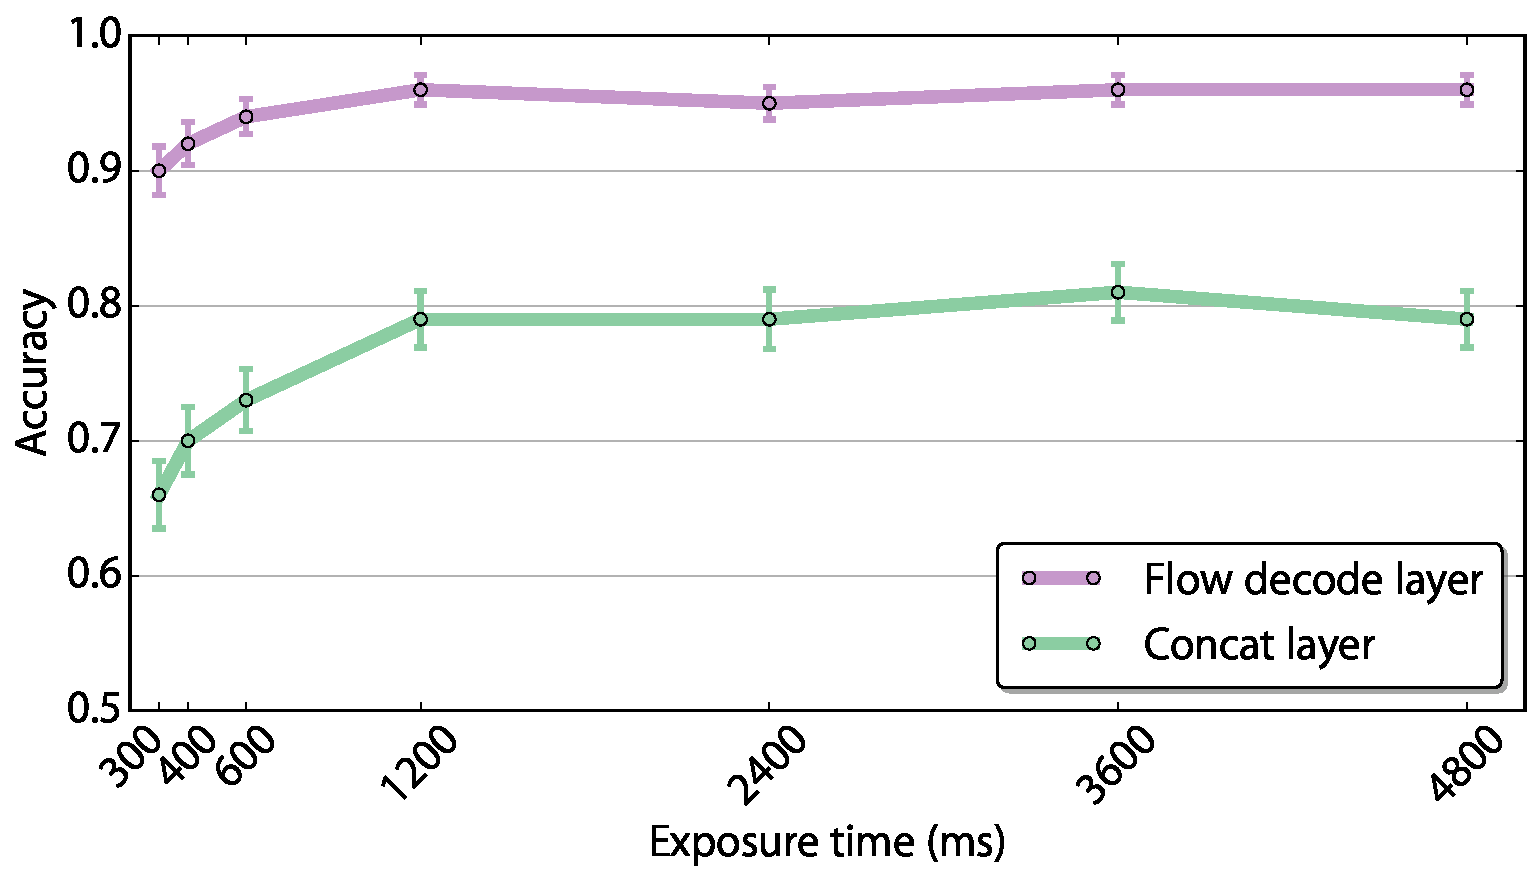
\epsfig{file=alltextures_approvedworkers.pdf, width = 0.9\textwidth}
	\caption[Time-limited pairwise comparisons across all textures]{Time-limited pairwise comparisons across all textures with $95\%$ statistical confidence intervals.}
	\label{fig:pairwise_alltextures}
\end{figure}



A full breakdown of the user study results by texture and 
grouping can be found in the supplemental material.
Here we discuss some of the overall trends.
Based on appearance it is clear that textures with
large-scale  spatial consistencies (regular, near-regular, 
and irregular textures) tend to perform poorly.
Examples being \texttt{flag} and \texttt{fountain\_2} with
user accuracies of $98.9\% \pm 1.6\%$ and $90.8\% \pm 4.3\%$ 
averaged across all exposures, respectively.
This is not unexpected and is a fundamental limitation of the 
local nature of the Gram matrix representation used in the 
appearance stream which was observed in static texture synthesis 
\cite{gatys2015}.
In contrast, stochastic and near-stochastic textures 
performed significantly better as their smaller-scale local 
variations are well captured by the appearance stream, for 
instance \texttt{water\_1} and \texttt{lava} which had 
average accuracies of $53.8\% \pm 7.4\%$ and
$55.6\% \pm 7.4\%$, respectively, making them both 
statistically indistinguishable from real.

\begin{figure}[t]
	\centering
	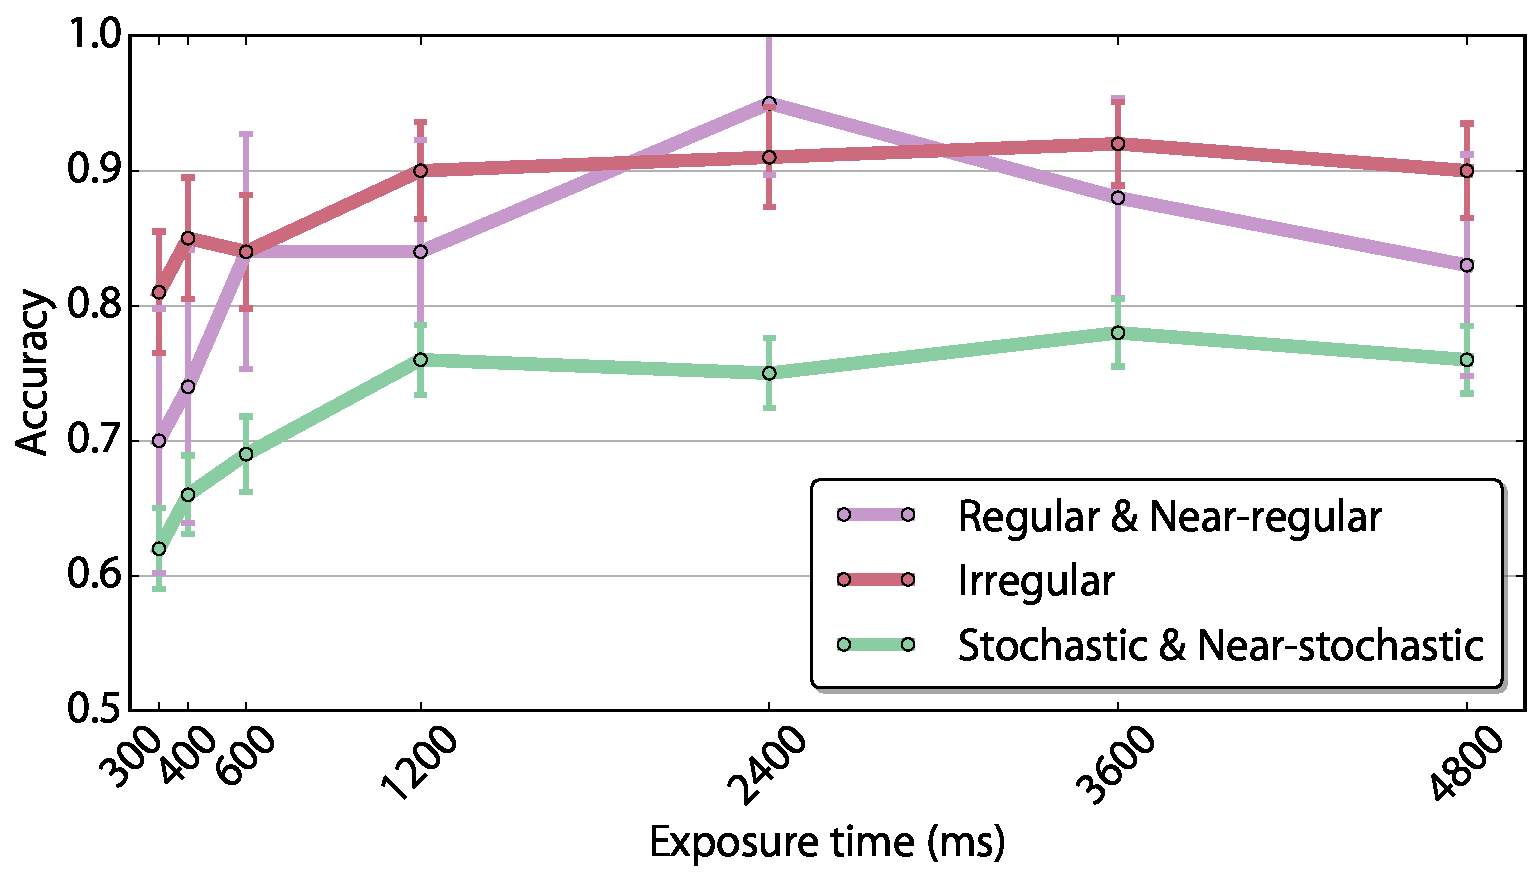
\epsfig{file=concat_appearance.pdf, width = 0.9\textwidth}\\
    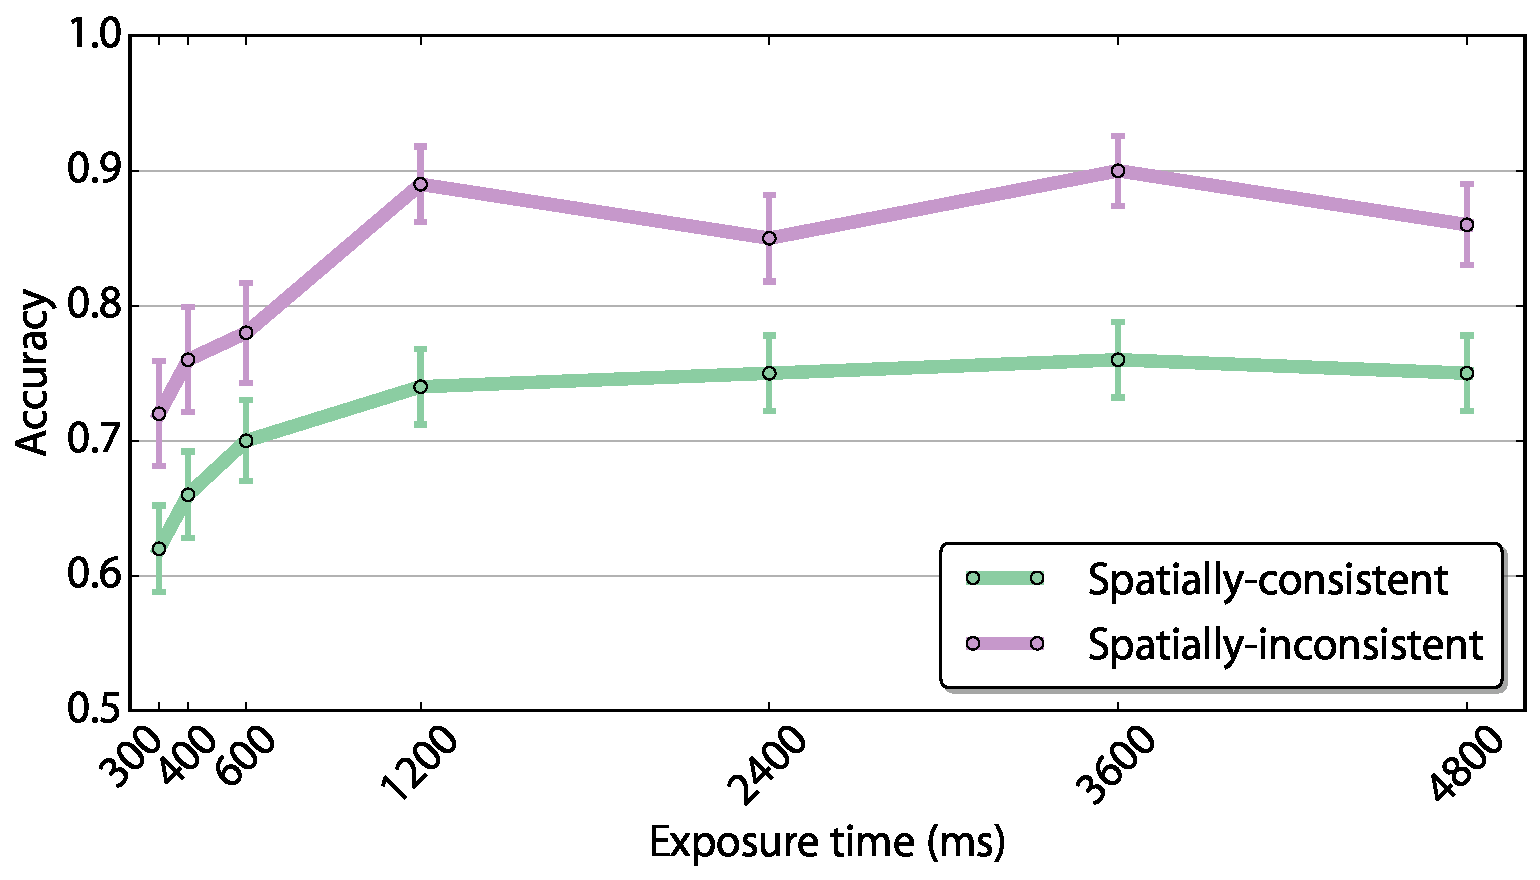
\epsfig{file=concat_dynamics.pdf, width = 0.9\textwidth}
	\caption[Time-limited pairwise comparisons across all textures, grouped by appearance and dynamics.]{Time-limited pairwise comparisons across all textures, grouped by appearance (top) and dynamics (bottom).  Shown with $95\%$ statistical confidence intervals.
	}
	\label{fig:pairwise_grouped}
	\vspace{-0.2cm}
\end{figure}

In terms of dynamics, we find that textures with
spatially-consistent dynamics (\eg, \texttt{tv\_static}, 
\texttt{water\_*}, and  \texttt{calm\_water\_*}) perform 
significantly better than those with spatially-inconsistent 
dynamics (\eg, \texttt{candle\_flame}, \texttt{fountain\_2}, 
and \texttt{snake\_*}), where the dynamics drastically differ 
across spatial locations.
For example, \texttt{tv\_static} and \texttt{calm\_water\_6}
have average accuracies of $48.6\% \pm 7.4\%$ and
$63.2\% \pm 7.2\%$, respectively, while
\texttt{candle\_flame} and \texttt{snake\_5} have average 
accuracies of $92.4\% \pm 4\%$ and $92.1\% \pm 4\%$, 
respectively.
Overall, our model is capable of reproducing a full spectrum
of spatially-consistent dynamics.
However, as the appearance shifts from containing small-scale 
spatial consistencies to containing large-scale consistencies,
performance degrades.
This was evident in the user study where the best-performing 
textures typically consisted of a stochastic or
near-stochastic appearance with spatially-consistent 
dynamics.
In contrast the worst-performing textures consisted of
regular, near-regular, or irregular appearance with
spatially-inconsistent dynamics.